\section{Разработка собственного технического решения}
\label{sec:---}
Как уже было описано ранее, в качестве датчика было решено выбрать потенциометрический датчик угла поворота.
К двум контактам датчика подключается источник опорного напряжения (10В), а на третьем формируется напряжение, величина которого зависит от угла поворота.

Так как измерительное устройство состоит из резистивных элементов большого номинала, в качестве источника опорного напряжения используем параметрический стабилизатор напряжения на стабилитроне.
\begin{figure}[!h]
    \centering
    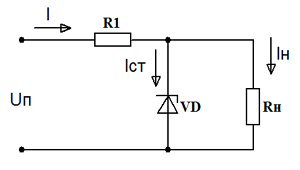
\includegraphics[width=0.5\textwidth]{img/img_4}
    \caption{Схема параметрического стабилизатора напряжения}
    \label{fig:img_4}
\end{figure}

В техническом задании указано, что диапазон измерения должен составлять от $\pm 5 ^\circ$.
Таким образом ширина диапазона измерений составляет $10^\circ$.
Изучение каталогов в поисках датчика с таким диапазоном измерений не привело к положительному результату: потенциометрические датчики угла поворота имеют больший допустимый угол поворота.
В связи с этим, необходимо использовать датчик с бОльшим диапазоном измерений, но использовать его только в требуемом.

\begin{figure}[!h]
    \centering
    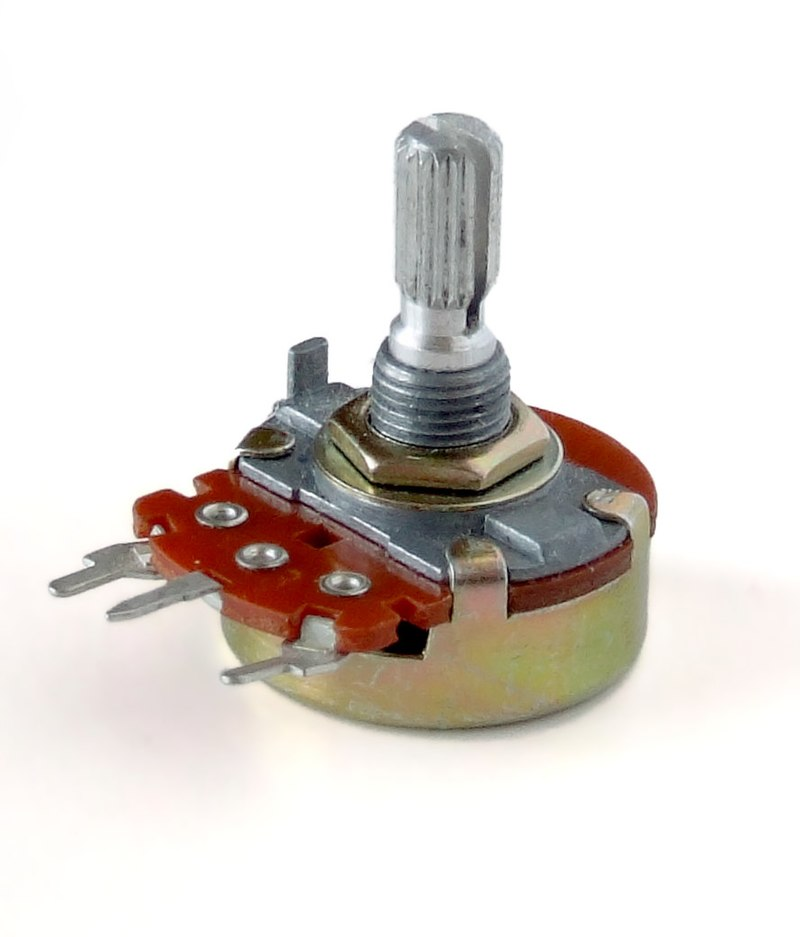
\includegraphics[width=0.4\textwidth]{img/img_3}
    \caption{Потенциометр B10K (WH148)}
    \label{fig:img3}
\end{figure}


Для примера рассмотрим вариант использования потенциометра B10K (WH148).
Его диапазон вращения составляет $300^\circ$.
Установим нулевую точку как поворот на $150^\circ$.
Соответственно, рабочим диапазоном потенциометра будет диапазон от $145^\circ$до $155^\circ$.
Минимальное и максимальное значение выходного напряжения потенциометра будет составлять:
\begin{gather*}
    U_{rout_{min}} = \frac{10\cdot145}{300}= 4.833\text{(В)}\\
    U_{rout_{max}} = \frac{10\cdot155}{300}= 5.167\text{(В)}
\end{gather*}
%https://chipenable.ru/index.php/how-connection/157-masshtabirovanie-signala-operacionnim-usilitelem.html

Это не соответствует заявленным требованиям.
Для решения возникшей проблемы воспользуемся масштабирующей схемой с операционным усилителем.

Выходное напряжение такой схемы считается по формуле:
\begin{gather*}
    U_{aout} = U_{ain}(1 + \frac{R_3}{R_2} + \frac{R_3}{R_1})-V_{cc}\frac{R_3}{R_1}
\end{gather*}

Выберем произвольное $R_3$ из ряда стандартных значений, например, 10кОм и рассчитаем номиналы $R_2$ и $R_1$ из системы уравнений:
\begin{gather*}
    \begin{cases}
        U_{aout_{min}} = U_{ain_{min}}(1 + \frac{R_3}{R_2} + \frac{R_3}{R_1})-V_{cc}\frac{R_3}{R_1}\\
        U_{aout_{max}} = U_{ain_{max}}(1 + \frac{R_3}{R_2} + \frac{R_3}{R_1})-V_{cc}\frac{R_3}{R_1}
    \end{cases}
\end{gather*}
\begin{gather*}
    \begin{cases}
        0 = 4.833(1 + \frac{10^4}{R_2} + \frac{10^4}{R_1})-10\frac{10^4}{R_1}\\
        10 = 5.167(1 + \frac{10^4}{R_2} + \frac{10^4}{R_1})-10\frac{10^4}{R_1}
    \end{cases}
\end{gather*}

\begin{gather*}
        R_1 = 6910.821\text{(Ом)}\ \
        R_2 = 6910.821\text{(Ом)}
\end{gather*}

Найдем ближайшие по номиналу стандартные значения:
\begin{gather*}
    R_1 = 6.8\text{(кОм)}\ \
    R_2 = 6.8\text{(кОм)}
\end{gather*}

Соберем схему измерительного устройства в программе LTspice и проведем моделирование:

\begin{figure}[!h]
    \centering
    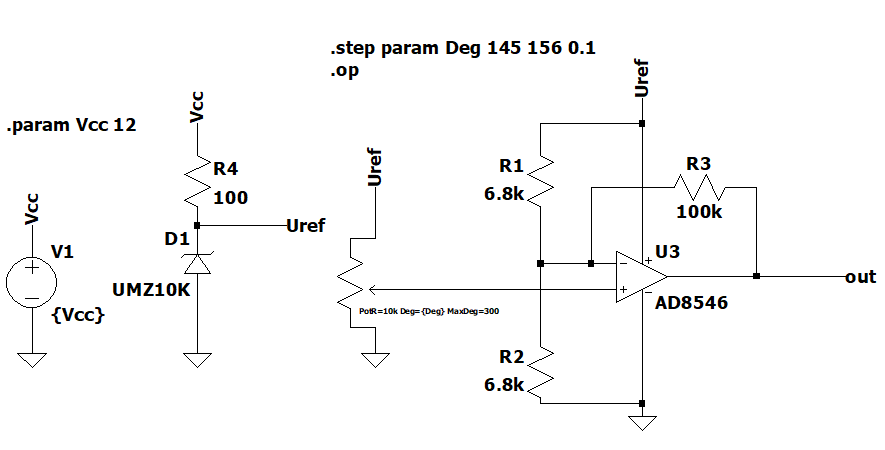
\includegraphics[width=0.7\textwidth]{img/img_5}
    \caption{Схема моделирования измерительного устройства}
    \label{fig:img_5}
\end{figure}
\newpage
\begin{figure}[!h]
    \centering
    \begin{minipage}{0.5\textwidth}
        \centering
        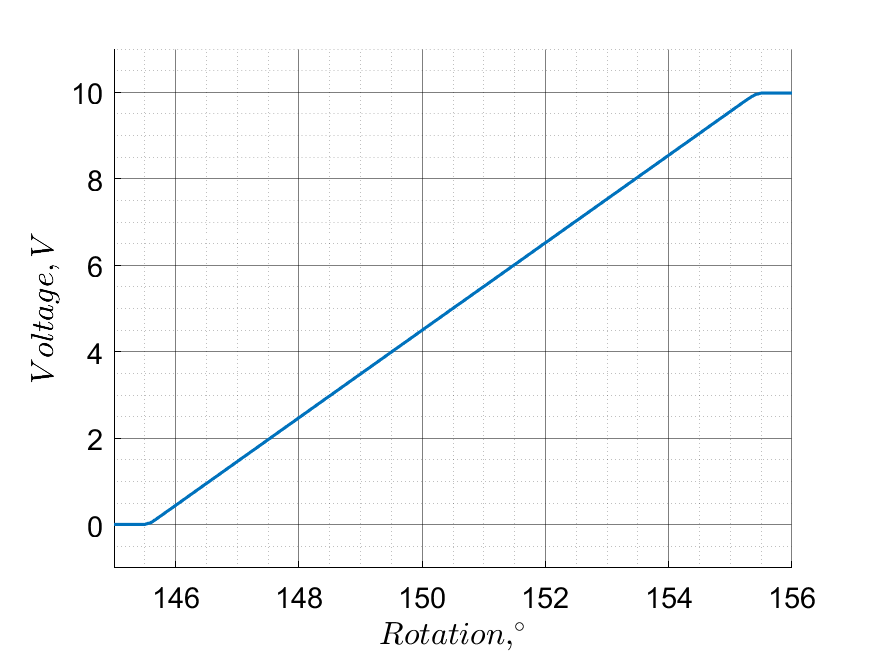
\includegraphics[width = 1\textwidth]{img/img_6}
        Без смещения
        \label{fig:img/img_5}
    \end{minipage}%
\begin{minipage}{0.5\textwidth}
        \centering
        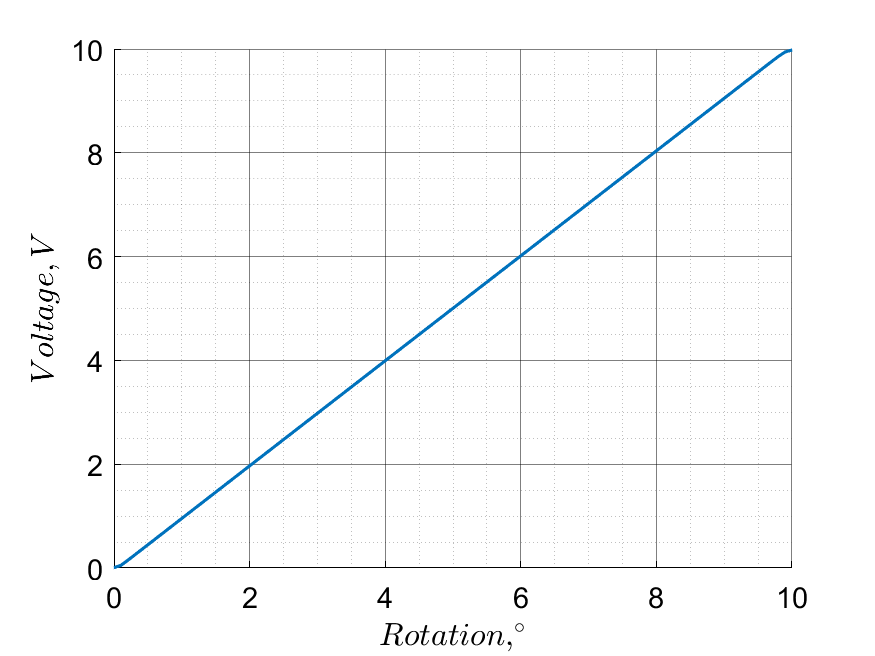
\includegraphics[width = 1\textwidth]{img/img_7}
        Со смещением
        \label{fig:img/img_7}
    \end{minipage}%
    \caption{Зависимость выходного напряжения от угла поворота}
\end{figure}

Как можно заметить, устройство соответствует техническому заданию: в диапазоне измерения $10\circ$ выходной сигнал (напряжение) изменяется в диапазоне 0--10В.

Остается выбрать источник питания: максимальное потребление схемы ограничено резистором $R_4$ (рисунок \ref{fig:img_5}):
\begin{gather*}
    P_{max} = U_{in}I_{max}\\
    I_{max} = \frac{U_{in}}{R_4}\\
    P_{max} = \frac{U^2_{in}}{R_4} = \frac{12^2}{100} = \frac{144}{100}=1.44(\text{Вт})
\end{gather*}
В связи с этим в качестве источника питания может быть выбран практически любой блок питания с ранее описанным напряжением 12В.
Например EPS-15-12 -- AC-DC блок питания со входным напряжением 85В -- 264В переменного тока и выходными 12В 1.25А постоянного (15Вт, что больше требуемого).
\begin{figure}[!h]
    \centering
    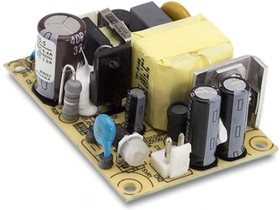
\includegraphics[width=0.5\textwidth]{img/img_8}
    \caption{Блок питания EPS-15-12}
    \label{fig:img_8}
\end{figure}

Выходной контакт измерительного устройства подключается к программируемому логическому контроллеру или микроконтроллеру, имеющему аналоговый вход с 10-вольтовым аналогово-цифровым преобразователем.
\newpage